\begin{answer}
Dataset 1 doesn't look like gaussian distribution. In my opinion, This is because $x2$ feature. I try to do log(x2) rather than original x2. This is the result.

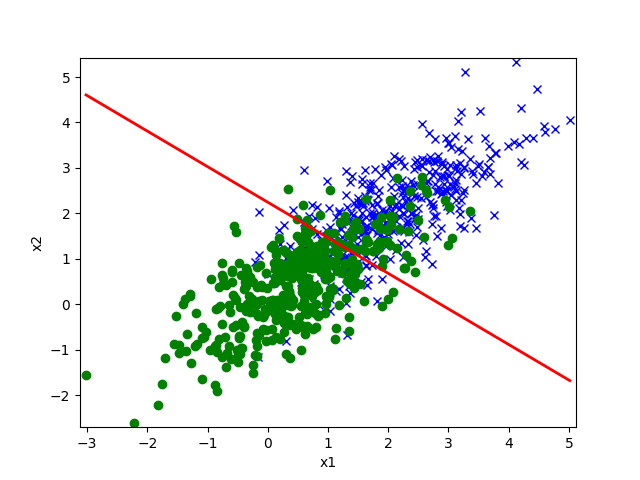
\includegraphics[width=0.5\textwidth]{linearclass/gda_plot_1_log_train.png}
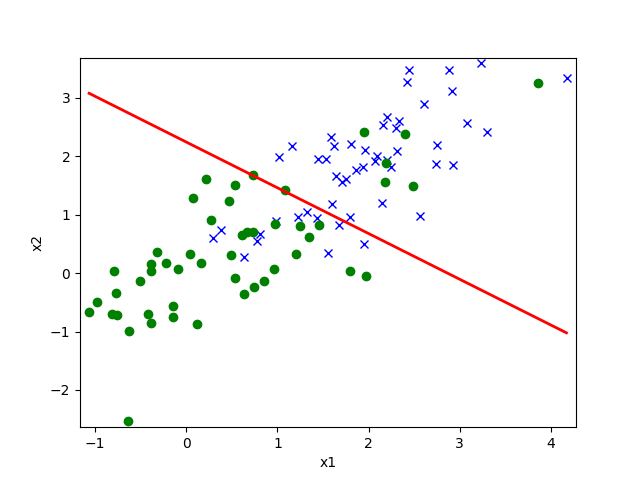
\includegraphics[width=0.5\textwidth]{linearclass/gda_plot_1_log_valid.png}

Train (left), valid (right)

As you can see, for now the distributions look like gaussian distribution and the boundary is better than original one.

\end{answer}
